\begin{enumerate}[label=\thesubsection.\arabic*,ref=\thesubsection.\theenumi]


\item Find the values of $k$ for which the line 
\begin{align}
(k-3)x-(4-k^2)y+k^2-7k+6=0 \label{eq:chapters/11/10/4/1/1}
\end{align}
is
\begin{enumerate}
\item Parallel to the $x$-axis
\item Parallel to the $y$-axis
\item Passing through the origin
\end{enumerate}
    \solution 
		The parameters of the given line are
\begin{align}
\vec{n}^{\top}\vec{x}=c \label{eq:chapters/11/10/4/1/2}
\end{align}
This equation can be expressed in the form of 
\begin{align}
\vec{n} = \myvec{k-3\\-4+k^2}, c  = -k^2+7k-6
\end{align}
\iffalse
Then \eqref{eq:chapters/11/10/4/1/1} can be expressed as
\begin{align}
\myvec{k-3 & -4+k^2}\vec{x} &=-k^2+7k-6\label{eq:chapters/11/10/4/1/4}
\end{align}
\fi
\begin{enumerate}
%part-1
    \item 
	    In this case,
	    \iffalse
The normal vector of $x$-axis is given by
\begin{align}
\myvec{0\\1}
\end{align}
\fi
equating $\vec{n}$ to the normal vector of $x$-axis,
\begin{align}
\myvec{k-3\\-4+k^2} &=\alpha\myvec{0\\1}\label{eq:chapters/11/10/4/1/6}
\\
\implies
k &=3
\end{align}
Substituting the value of $k$ in \eqref{eq:chapters/11/10/4/1/1}, the desired equation is
\begin{align}
        \myvec{0 & 5}\vec{x} &=6
\end{align}

\item In this case, 
equating $\vec{n}$ to the normal vector of $y$-axis,
\begin{align}
\myvec{k-3\\-4+k^2} &=\beta\myvec{1\\0}\label{eq:chapters/11/10/4/1/11}
\\
	\implies k &=\pm2
\end{align}
Substituting the value of $k$ in \eqref{eq:chapters/11/10/4/1/1}, the desired equation is 
\begin{align}
        \myvec{-1 & 0}\vec{x} &=4, \quad  k &=2\\
        \myvec{-5 & 0}\vec{x} &=-24, \quad  k &=-2
\end{align}
\item 
	In this case, 
\begin{align}
	c = 0 \implies 
	-k^2+7k-6 &= 0\\
	\implies k =1 \text{ or } k&=6
\end{align}
Substituting the value of $k$ in \eqref{eq:chapters/11/10/4/1/1}, the desired equations are 
\begin{align}
        \myvec{-2 & -3}\vec{x} &=0, \quad  k &=1\\
       \myvec{3 & 32}\vec{x} &=0, \quad  k &=6
\end{align}
\end{enumerate}

	\item Find the  equations of the lines, which cutoff intercepts on the axes  whose sum and product are 1 and -6 respectively.
\\
\solution
		Let the intercepts be $a$ and  $b$. Then
\begin{align}
a+b=1,
ab=-6 \label{eq:11/10/4/32a}
\\
\implies  a = 3, b = -2
\end{align}
Thus, the possible 
intercepts are
\begin{align}
\myvec{3\\0}, \myvec{0\\-2},
\myvec{-2\\0}, \myvec{0\\3}
\end{align}
From
		\eqref{prop:lin-eq-unit-mat},
\begin{align}
	\myvec{3 & 0 \\ 0 &-2}\vec{n} = \myvec{1 \\ 1}
	\\
	\implies \vec{n} = \myvec{\frac{1}{3} \\ -\frac{1}{2}}
	\\
	\text{or, } \myvec{2 & -3}\vec{x} = 6
\end{align}
using		\eqref{prop:lin-eq-unit}.
Similarly, the other line can be obtained
as
\begin{align}
	\myvec { 3 & -2 }  \vec{x}  = -6        
\end{align}
See  
\figref{fig:11/10/4/3line segmenta}.
\begin{figure}[!htbp]
\centering
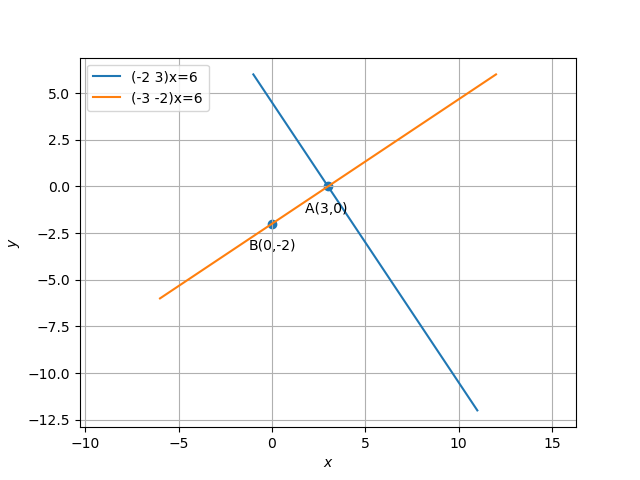
\includegraphics[width=\columnwidth]{chapters/11/10/4/3/figs/inter.png}
\caption{}
\label{fig:11/10/4/3line segmenta}
\end{figure}

\item A ray of light passing through the point $\vec{P} = \brak{1, 2}$ reflects on the x-axis at point $\vec{A}$ and the reflected ray passes through the point $\vec{Q} =\brak{5, 3}$. Find the coordinates of $\vec{A}$.
\\
    \solution 
			From \eqref{eq:11/10/4/22},
the reflection of $\vec{Q}$ is 
\begin{align}
\vec{R}  
= \myvec{5\\-3}
\end{align}
Letting
\begin{align}
\vec{A} = \myvec{x\\0},
\end{align}
since 
$\vec{P},
\vec{A},  
\vec{R}  
$
are collinear, 
		from \eqref{prop:lin-dep-rank},
\begin{align}
	\myvec{
		1 & 1 & 2 
		\\ 
		1 & 5 & -3 
		\\
		1 & x & 0 }
	\xleftrightarrow[R_3=R_3 - R_1]{R_2 = R_2 - R_1}
	\myvec{
		1 & 1 & 2 
		\\ 
		0 & 4 & -5 
		\\
		0 & x-1 & -2 }
	\\
	\xleftrightarrow[]{R_3 = 4R_3 - \brak{x-1}R_2}
	\myvec{
		1 & 1 & 2 
		\\ 
		0 & 4 & -5 
		\\
		0 & 0 & 5x-13 }
	\implies x = \frac{13}{5}
\end{align}
See  
\figref{fig:chapters/11/10/4/22/1}.
\begin{figure}[H]
\centering
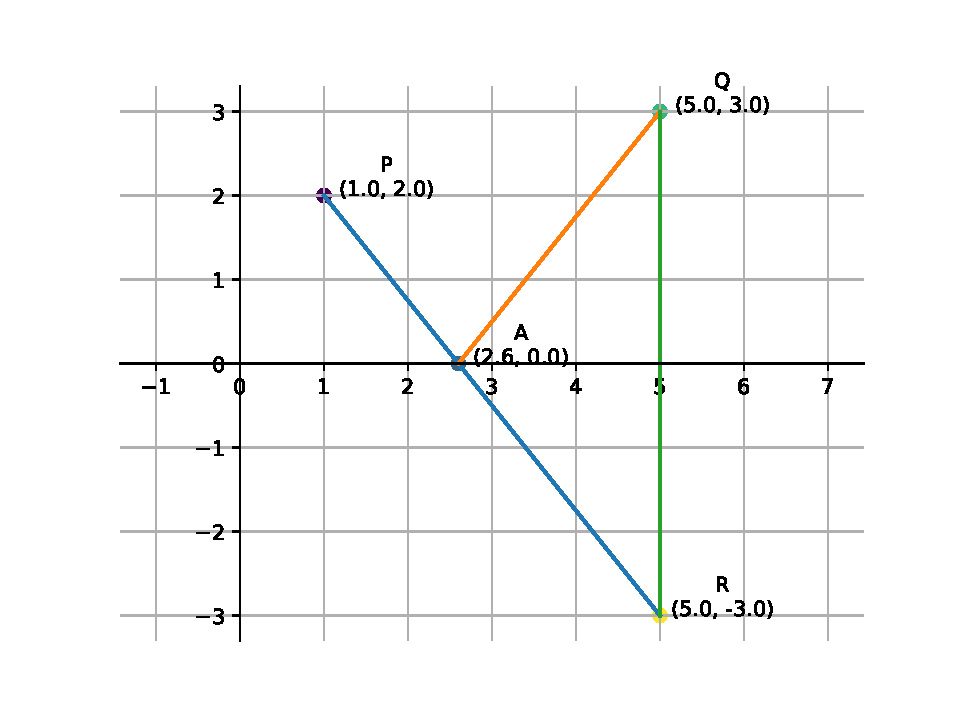
\includegraphics[width=0.75\columnwidth]{chapters/11/10/4/22/figs/fig.pdf}
\caption{}
\label{fig:chapters/11/10/4/22/1}
\end{figure}




\item Prove that in any $\triangle{ABC}$, cos A=$\frac{b^2+c^2-a^2}{2bc}$, where a,b,c are the magnitudes of the sides opposite to the vertices A,B,C respectively.
\item Distance of the point $(\alpha, \beta, \gamma)$ from y-axis is
\begin{enumerate}
	\item $\beta$ 
	\item $\abs{\beta}$
	\item $\abs{\beta+\gamma}$
	\item $\sqrt{\alpha^2+\gamma^2}$
\end{enumerate}
\item The reflection of the point $(\alpha, \beta, \gamma )$ in the xy-plane is 
\begin{enumerate}
	\item $\alpha,\beta,0)$
	\item $(0,0,\gamma)$
	\item $(-\alpha,-\beta,\gamma)$
	\item $(\alpha,\beta,-\gamma)$
\end{enumerate}
\item The plane $ax+by=0$ is rotated about its line of intersection with the plane $z=0$ through an angle $\alpha.$ Prove that the equation of the plane in its new position is $ax+by \pm (\sqrt{a^2+b^2} \tan\alpha)z=0.$
\item The locus represented by $xy+yz=0$ is 
\begin{enumerate}
	\item A pair of perpendicular lines
	\item A pair of parallel lines
	\item A pair of parallel planes 
	\item A pair of perpendicular planes
\end{enumerate}
\item Find the equation of the straight line which passes through the point (1, -2) and cuts off equal intercepts from axes.
\item Find the equation of the line passing through the point (5,2) and perpendicular to the line joining the points (2,3) and (3, -1).
\item Find the angle between the lines $y(2-\sqrt{3})(x+5)\text{ and }y=(2+\sqrt{3})(x-7)$.
\item Find the equation of the lines which passes the point (3,4) and cuts off intercepts from the coordinate axes such that their sum is 14.
\item Find the points on the line $x+y=4$ which lie at a unit distance from the line $4x+3y=10$.
\item Show that the tangent of an angle between the lines $\frac{x}{a}+\frac{y}{b}=1 \text{ and }\frac{x}{a}-\frac{y}{b}=1$ is $\frac{2ab}{a^2-b^2}$.
\item Find the equation of lines passing through (1,2) and making angle $30\degree$ with $y$-axis.
\item Find the equation of the line passing through the point of intersection of $2x+y=5\text{ and }x+3y+8=0$ and parallel the line $3x+4y=7$.
\item For what values of $a$ and $b$ the intercepts cut off on the coordinate axes by the line $ax+by+8=0$are equal in length but opposite in signs to those cut off by the line $2x-3y+=0$ on the axes.
\item If the intercept of a line between the coordinate axes is divided by the point (-5,4) in the ratio 1:2 then find the equation of the line.
\item Find the equation of a straight line on which length of perpendicular from the origin is four units and the line makes on angle of 120$\degree$ with the positive direction of $x$-axis. [\textbf{Hint} : Use normal form, here $\omega =30\degree$.]
\item Find the equation of one of the sides of an isosceles right angled triangle whose hypotenuse is given by $3x+4y=4$ and the opposite vertex of the hypotenuse is (2,2).
\end{enumerate}
 \textbf{Long Answer Type}
 \begin{enumerate}[resume]
\item If the equation of the base of an equilateral triangle is $x+y=2$ and the vertex is (2,-1), then find the length of the side of the triangle. 
[\textbf{Hint} : Find length of perpendicular ($p$) from (2,-1) to the line and use $p=l \sin 60degree$,where $l$ is the length of the triangle].
\item A variable line passes through a fixed point $\vec{P}$.The algebraic sum of the perpendiculars drawn from the points (2,0),(0,2) and (1,1) on the line is zero. Find the coordinates of the point $\vec{P}$.  
[\textbf{Hint} : let the slope of the line be $m$. Then the equation of the line passing through the fixed point $\vec{P}(x_1,y_1) y-y_1=m(x-x_1)$. Taking the algebraic sum of perpendicular distances equal to zero, we get $y-l=m(x-1)$. Thus $(x_1,y_1)$ is (1,1).]
\item In what direction should a line be drawn through the point (1,2) so that its point of intersection with line $x+y=4$ is at a distance $\sqrt{6}{3}$ from the given equilateral    
\item A straight line moves so that the sum of the reciprocals of its intercepts made on axes is constant. Show that the line passes through a fixed point. [\textbf{Hint} : $\frac{x}{a}+\frac{y}{b}=1\text{ where} \frac{1}{a}+\frac{1}{b}=\text{ constant }=\frac{1}{k}$(say). This implies that $\frac{k}{a}+\frac{k}{b}=1$ line passes through the fixed point $(k,k)$.]
\item Find the equation of the line which passes through the point (-4,3) and the portion of the line intercepted between the axes is divided internally in ratio 5:3 by this point.
\item Find the equations of the lines through the point of intersection of the line $x-y+1=0 \text{ and }2x-3y+5=0$ and whose distance from the point (3,2) is $\frac{7}{5}$.
\item If the sum of the distances of a moving point in a plane from the axes is $l$, then finds the locus of the point. [\textbf{Hint} :Given that $\abs{x}+\abs{y}=1$, which  gives four  sides of a square.] 
\item $\vec{P}_1,\vec{P}_2$ are points on either of the two lines $y-\sqrt{3}\abs{x}=2$ at a distance of 5 units from their point of intersection. Find the coordinates of the root of perpendiculars drawn from $P_1, P_2$ on the bisector of the angle between the given lines.
[\textbf{Hint} : Lines are $y=\sqrt{3}x+2 \text{ and }y=-\sqrt{3}x+2$ according as $x\geq0$ or $x0. y$-xis is the bisector of the angles between the lines. $P_1, P_2$ are the points on these lines at a distance of 5 units from the point of intersection of these lines which have a point on $y$-axis as a common foot of perpendiculars from these points. The $y$-coordinate of the foot of the perpendicular is given by 2=5 $\cos{30\degree}$.]
\item If $p$ is the length of perpendicular from the origin on the lien $\frac{x}{a}+\frac{y}{b}=1$ and $a^2,p^2,b^2$ are in A.P, then show that $a^4+b^4=0$.
\end{enumerate}
\textbf{Objective Type Questions}\\
choose the correct answer from the given four options in Exercises 22 to 41
\begin{enumerate}[resume]
\item A line cutting off intercept -3 from the tangent at angle to the $x$-axis is $\sqrt{3}{5}$, its equation is
\begin{enumerate}
\item $5y-3x+15=0$
\item $3y-5x+15=0$
\item $5y-3x-15=0$
\item none of these
\end{enumerate}
\item Slope of a line which cuts off intercepts of equal length on the axes is 
\begin{enumerate}
\item -1
\item -0
\item 2
\item $\sqrt{3}$
\end{enumerate}
\item The equation of the straight line passing through the point (3,2) and perpendicular to the line $y=x$ is
\begin{enumerate}
\item $x-y=5$
\item $x+y=5$
\item $x+y=1$
\item $x-y=1$
\end{enumerate}
\item The equation of the line passing through the point (1,2) and perpendicular to the line $x+y+1=0$ is
\begin {enumerate}
\item $y-x+1=0$
\item $y-x-1=0$
\item $y-x+2=0$
\item $y-x-1=0$
\end{enumerate}
\item The tangent of angle between the lines whose intercepts on the axes are $a,-b$ and $b,-a$, respectively, is
\begin{enumerate}
\item $\frac{a^2-b^2}{ab}$
\item $\frac{b^2-a^2}{2}$
\item $\frac{b^2-a^2}{2ab}$
\item none of these 
\end{enumerate}
\item If the line $\frac{x}{a}+\frac{y}{b}=1$ passes the points (2,-3) and (4,-5), then $(a,b)$ is 
\begin{enumerate}
\item (1,1)
\item (-1,1)
\item (1,-1)
\item (-1,-1)
\end{enumerate}
\item The distance of the point of intersection of the lines $2x-3y+5=0 \text{ and }3x+4y=0$ from the line $5x-2y=0$ is
\begin{enumerate}
\item $\frac{130}{17\sqrt{29}}$
\item $\frac{13}{7\sqrt{29}}$
\item $\frac{130}{7}$
\item none of these
\end{enumerate}
\item The equations of the lines which pass through the point (3, -2) and are inclined at $60\degree$ to the line $\sqrt{3} x+y=1$ is
\begin{enumerate}
\item $y+2=0$, $\sqrt{3}x-y-2-3\sqrt{3}=0$
\item $x-2=0$, $\sqrt{3}x-y+2+3\sqrt{3}=0$
\item $\sqrt{3}x-y-2-3\sqrt{3}=0$
\item None of these
\end{enumerate}
\item The equations of the lines passing through the point (1,0) and at a distance $\frac{\sqrt{3}}{2}$ from the origin, are 
\begin{enumerate}
\item $\sqrt{3}x+y-\sqrt{3}=0$, $\sqrt{3}x-y-\sqrt{3}=0$
\item $\sqrt{3}x+y+\sqrt{3}=0$, $\sqrt{3}x-y+\sqrt{3}=0$
\item $x+\sqrt{3}y-\sqrt{3}=0$, $\sqrt{3}y-\sqrt{3}=0$
\item None of these.
\end{enumerate}
\item The distance between the lines $y=mx+c$,\text{ and }$y=mx+c^2$ is
\begin{enumerate}
\item $\frac{c_1-c_2}{\sqrt{m+1}}$
\item $\frac{\abs{c_1-c_2}}{\sqrt{1+m^2}}$
\item $\frac{c^2-c^1}{\sqrt{1+m^2}}$
\item 0
\end{enumerate}
\item The coordinates of the foot of perpendiculars from the point (2,3) on the line $y=3x+4$ is given by 
\begin{enumerate} 
\item $\frac{37}{10}$, $\frac{-1}{10}$
\item $\frac{-1}{10}$, $\frac{37}{10}$
\item $\frac{10}{37}$, -10
\item $\frac{2}{3}$, $\frac{-1}{3}$
\end{enumerate}
\item If the coordinates of middle point of the portion of a line intercepted between the coordinate axes is (3,2),then the equation of the line will be
\begin{enumerate}
\item $2x+3y=12$
\item $3x+2y=12$
\item $4x-3y=6$
\item $5x-2y=10$
\end{enumerate}
\item Equation of the line passing through (1,2) and parallel to the line $y=3x-1$ is
\begin{enumerate}
\item $y+2=x+1$
\item $y+2=3(x+1)$
\item $y-2=3(x-1)$
\item $y-2=x-1$
\end{enumerate}
\item Equations of diagonals of the square formed by the lines $x=0$, $y=0$, $x=1$ and $y=1$ are
\begin{enumerate}
\item $y=x$, $y+x=1$
\item $y=x$,$x+y=2$
\item $2y=x$, $y+x=\frac{1}{3}$
\item $y=2x$, $y+2x=1$
\end{enumerate}
\item For specifying a straight line, how many geometrical parameters should be known?
\begin{enumerate}
\item 1
\item 2
\item 4
\item 3
\end{enumerate}
\item The point (4,1)undergoes the following two successive transformations :
\begin{enumerate}
\item Reflection about the line $y=x$
\item Translation through a distance 2 units along the positive $x$-axis 
\end{enumerate}
Then the final coordinates of the point are
\begin{enumerate}
\item (4,3)
\item (3,4)
\item (1,4)
\item $\frac{7}{2}$,$\frac{7}{2}$
\end{enumerate}
\item A point equidistant from the lines $4x+3y+10=0$, $5x-12y+26=0$ and $7x+24y-50=0$ is
\begin{enumerate}
\item (1,-1)
\item (1,1)
\item (0,0)
\item (0,1)
\end{enumerate}
\item A line passes through (2,2) and is perpendicular to the line $3x+y=3$. Its $y$-intercept is 
\begin{enumerate}
\item $\frac{1}{3}$
\item $\frac{2}{3}$
\item 1
\item $\frac{4}{3}$
\end{enumerate}
\item The ratio in which the line $3x+4y+2=0$ divides the distance between the lines $3x+4y+5=0$ and $3x+4y-5=0$ is
\begin{enumerate}
\item 1:2
\item 3:7
\item 2:3
\item 2:5
\end{enumerate}
\item One vertex of the equilateral with centroid at the origin and one side as $x+y-2=0$ is
\begin{enumerate}
\item (-1,-1)
\item (2,2)
\item (-2-2)
\item (2,-2)
\end{enumerate}
[\textbf{Hint} : Let $ABC$ be the equilateral triangle with vertex $\vec{A}(h,k)\text{ and let }\vec{D}(\alpha,\beta)$ be the point on $BC$. Then $\frac{2\alpha+h}{3}=0=\frac{2\beta+k}{3}$. Also ${\alpha+\beta-2=0}\text{ and }\frac{k-0}{h-o}x(-1)=-1$] 
\end{enumerate}

Fill in the blank in Exercises 42 to 47.
\begin{enumerate}[resume]
\item If $a,b,c$ are is A.P.,then the straight lines $ax+by+c=0$ will always pass through \rule{1cm}{0.15mm}.
\item The line which cuts off equal intercept from the axes and pass through the equilateral2) is \rule{1cm}{0.15mm}.
\item Equations of the lines through the point (3,2) and making an angle of $40\degree$ with the line $x-2y=3$ are \rule{1cm}{0.15mm}.   
\item The points (3,4) and (2,-6)are situated on the \rule{1cm}{0.15mm} of the line $3x-4y-8=0$.
\item A point moves so that square of its distance from the point (3,-2) is numerically equal to its distance from the line $5x-12y=3$. The equation of its locus is %\rule{1cm}{0.15mm}.
\item Locus of the mid-points of the portion of the line $x\sin\theta+y\cos\theta=p$ intercepted between the axes is \rule{1cm}{0.15mm}.
State whether the statements in Exercises 48 to 56 are true or false. Justify.
\item If the vertices of a triangle have integral coordinates, then the triangle can not be equilateral.
\item The points $\vec{A}(2,1)$, $\vec{B}(0,5)$, $\vec{C}(-1,2)$ are collinear.
\item Equation of the line passing through the point $(a\cos^3\theta, a\sin^3\theta)$ and perpendicular to the line $x\sec\theta+y\csc\theta=a$ is $x\cos\theta-y\sin\theta=\alpha\sin2\theta$.
\item The straight line $5x+4y=0$ passes through the point of intersection of the straight lines $x+2y-10=0$ and $2x+y+5=0$.
\item The vertex of on equilateral triangle is (intercepted equation of the opposite side is $x+y=2$.then the other two sides are $y-3=(2\pm\sqrt{3})(x-2)$.
\item The equation of the line joining the point (3,5) to the point of intersection of the lines $4x+y-=0$ and $7x-3y-5=0$ is equidistant from the points (0,0) and (8,34).
\item The line $\frac{x}{a}+\frac{y}{b}=1$ moves in such a way that $\frac{1}{a^2}+\frac{1}{b^2}=\frac{1}{c^2}$, where $c$ is a constant.The locus of the foot of the perpendicular from the origin on the given line is $x^2+y^2=c^2$.
\item The lines $ax+2y+1=0$, $bx=3y+1=0\text{ and }cx+4y+1=0$ are concurrent if $a$, $b$, $c$ are in G.P.
\item Line joining the points (3,-4) and (-2,6) is perpendicular to the line joining the points (-3,6) and (9,-18).
\end{enumerate}
Match the questions given under Column $C_1$ with their appropriate answers given under the Column $C_2$ is Exercises 57 to 59.
\begin{enumerate}[resume]
\item 
\begin{center}
\begin{tabular}{cccccc}
\textbf{Column $C_1$} & & & & &  \textbf{Column $C_2$}\\
\end{tabular}   
\end{center}
\begin{matchtabular}
  The coordinates of the points P and Q on the line x + 5y = 13 which are at a distance of 2 units from the line 12x – 5y + 26 = 0 are & (3,1),(-7,11)\\
  The coordinates of the point on the line x + y = 4, which are at a unit distance from the line 4x + 3y – 10 = 0 are & $-\frac{1}{11},\frac{11}{3}$ , $\frac{4}{3},\frac{7}{3}$\\
  The coordinates of the point on the line joining A (–2, 5) and B (3, 1) such that AP = PQ = QB are & 1,$\frac{12}{5}$ , $-3,\frac{16}{5}$\\
\end{matchtabular}
\\
\item The value of the $\lambda$, if the lines\\$(2x+3y+4)+\lambda(6x-y+12)=0$ are
\begin{center}
\begin{tabular}{cccccc}
\textbf{Column $C_1$} & & & & &  \textbf{Column $C_2$}\\
\end{tabular}   
\end{center}
\begin{matchtabular}
parallel to $y$-axis is & $\lambda =-\frac{3}{4}$\\
perpendicular to $7x+y-4=0$ is & $\lambda=-\frac{1}{3}$\\
passes through (1,2) is & $\lambda=-\frac{17}{41}$\\
parallel to $x$ axis is & $\lambda=3$\\
\end{matchtabular}
\\
\item The equation of the line through the intersection of the lines $2x-3y=0$ and $4x-5y=2$ and
\begin{center}
\begin{tabular}{cccccc}
\textbf{Column $C_1$} & & & & &  \textbf{Column $C_2$}\\
\end{tabular}   
\end{center}

\begin{matchtabular}
through the point (2,1) is & $2x-y=4$\\
perpendicular to the line & $x+y-5=0$\\
parallel to the line $3x-4y+5=0$ is & $x-y-1=0$\\
equally inclined to the axes is & $3x-4y-1=0$\\
\end{matchtabular}
\end{enumerate}
